\documentclass[11pt]{article}
\usepackage[a4paper,margin=2.4cm]{geometry}
\usepackage[T1]{fontenc}
\usepackage{lmodern}
\usepackage{microtype}
\usepackage{xcolor}
\usepackage{booktabs}
\usepackage{pgfplots}
\pgfplotsset{compat=1.18}
\usepackage[colorlinks,linkcolor=blue!60!black,urlcolor=blue!60!black]{hyperref}
\usepackage{bookmark}
\definecolor{river}{HTML}{3559E0}
\definecolor{moss}{HTML}{4C9A5B}
\definecolor{clay}{HTML}{D2683A}
\title{\textbf{Mountain Streams}\\[4pt]\large A short field guide for weekend walkers}
\author{Field Notes Series, No.~7}
\date{Spring edition}
\begin{document}
\maketitle

\begin{abstract}
Mountain streams change from hour to hour. Snow melts in the afternoon, storms
arrive without warning and a calm pool in the morning can be a torrent by
evening. This guide explains how to read a stream, how to measure its flow with
nothing more than a stopwatch and a stick, and how to cross one safely.
\end{abstract}

\tableofcontents

\section{Reading a stream}

A stream tells you a lot about itself if you know where to look. The colour of
the water, the sound it makes and the stones on its bed all hint at how fast it
is moving and how deep it is.

\subsection{Pools, riffles and runs}

Most streams repeat the same three shapes. \emph{Pools} are deep, slow and dark;
\emph{riffles} are shallow stretches where the water breaks white over stones;
\emph{runs} join the two, smooth on the surface but quick underneath. Trout rest
in pools and feed at the head of riffles, where the current brings them insects.

\subsection{The colour of the water}

Clear water usually means a stable bed and low flow. Milky, blue-grey water
comes from glaciers and carries fine rock flour. Brown water after rain means
the stream is carrying soil, and is rising: treat it with care.

\section{Measuring the flow}

You can estimate how much water a stream carries with the \emph{float method}.
Mark two points ten metres apart along a straight stretch, drop a stick in the
water upstream and time how long it takes to pass between the marks. Multiply
the speed by the width and the average depth to get the flow in cubic metres per
second.

\begin{center}
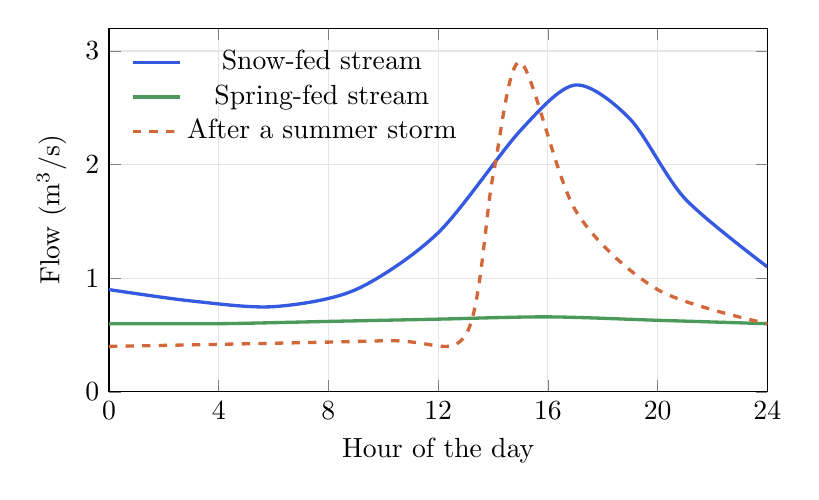
\begin{tikzpicture}
\begin{axis}[
  width=0.82\textwidth, height=6.2cm,
  xlabel={Hour of the day}, ylabel={Flow (m$^3$/s)},
  xmin=0, xmax=24, ymin=0, ymax=3.2,
  xtick={0,4,8,12,16,20,24},
  grid=major, grid style={gray!20},
  legend style={at={(0.02,0.97)},anchor=north west,draw=none,fill=none},
  every axis plot/.append style={very thick},
]
\addplot[river, smooth] coordinates {(0,0.9) (3,0.8) (6,0.75) (9,0.9) (12,1.4) (15,2.3) (17,2.7) (19,2.4) (21,1.7) (24,1.1)};
\addlegendentry{Snow-fed stream}
\addplot[moss, smooth] coordinates {(0,0.6) (4,0.6) (8,0.62) (12,0.64) (16,0.66) (20,0.63) (24,0.6)};
\addlegendentry{Spring-fed stream}
\addplot[clay, smooth, dashed] coordinates {(0,0.4) (10,0.45) (13,0.5) (14,1.9) (15,2.9) (17,1.6) (20,0.9) (24,0.6)};
\addlegendentry{After a summer storm}
\end{axis}
\end{tikzpicture}
\end{center}

Snow-fed streams peak in the late afternoon, when the day's meltwater arrives.
Cross them in the morning. Spring-fed streams barely change at all, while a
storm can raise any stream within minutes.

\section{Crossing safely}

\subsection{Choosing a place}

Look for a wide, straight stretch where the water is slow and shallow. Avoid the
outside of bends, where the current is strongest, and never cross just above a
waterfall or a log jam.

\subsection{How deep is too deep?}

\begin{center}
\begin{tabular}{@{}llll@{}}
\toprule
Depth & Slow water & Fast water & Advice \\
\midrule
Ankle & Easy & Easy & Keep boots on for grip \\
Knee & Easy & Difficult & Use a pole, face upstream \\
Thigh & Difficult & Dangerous & Cross as a group, or wait \\
Waist & Dangerous & Do not cross & Turn back \\
\bottomrule
\end{tabular}
\end{center}

Unclip the hip belt of your rucksack before you step in, so you can drop it if
you fall. Move one foot at a time and always keep two points of contact with the
bed, counting the pole.

\subsection{If you fall in}

Float on your back with your feet pointing downstream and near the surface, so
they can push you off rocks. Do not try to stand up in fast water: a foot caught
between stones can hold you under. Swim towards the bank at an angle once the
current slows.

\section{Leaving no trace}

Streams are home to insects, fish and the birds that feed on them. Wash dishes
and yourself at least sixty metres from the water, carry out everything you
carry in, and step on stones rather than the soft bank, which collapses easily
and muddies the water for everything living downstream.

\section{Checklist}

\begin{itemize}
\item Check the weather and the snow report the night before.
\item Plan to cross snow-fed streams before noon.
\item Bring a walking pole and dry socks in a waterproof bag.
\item Tell someone where you are going and when you will be back.
\end{itemize}

\end{document}
